% !TeX program = xelatex
\documentclass[11pt,a4paper]{article}

\usepackage[vietnamese]{babel}
\usepackage{fontspec}
% Dùng duy nhất một họ font serif hỗ trợ Unicode tiếng Việt cho toàn bài.
\setmainfont{TeX Gyre Termes}
\setsansfont{TeX Gyre Termes}
\setmonofont{TeX Gyre Termes}
\usepackage{microtype}
\usepackage{geometry}
\usepackage{booktabs}
\usepackage{array}
\usepackage{amsmath}
\usepackage{amssymb}
\usepackage{unicode-math}
\setmathfont{TeX Gyre Termes Math}
\usepackage{graphicx}
\usepackage{xcolor}
\usepackage{hyperref}
\usepackage{enumitem}
\usepackage{caption}
\usepackage{float}
\usepackage{listings}
\usepackage{tikz}
\usetikzlibrary{arrows.meta,positioning,shapes.geometric}

\geometry{top=22mm,bottom=24mm,left=23mm,right=23mm}
\hypersetup{colorlinks=true,linkcolor=teal!60!black,citecolor=teal!60!black,urlcolor=blue!60!black}
\setlength{\parindent}{1.2em}
\setlength{\parskip}{0.25em}
\renewcommand{\arraystretch}{1.15}
\lstset{basicstyle=\ttfamily\small,breaklines=true,frame=single,columns=fullflexible}

\title{\textbf{xFace: Hệ thống Edge AI phát hiện, nhận diện và điểm danh khuôn mặt thời gian thực trên Luckfox RV1106}}
\author{Võ Quốc Kha \and Trần Ngọc Tú \and Huỳnh Đăng Khoa}
\date{Tháng 8 năm 2026}

\begin{document}
\maketitle

\begin{abstract}
Nghiên cứu trình bày xFace, một hệ thống Edge AI điểm danh khuôn mặt thời gian thực trên Luckfox RV1106. Thành phần trung tâm là YOLOv5s được train từ 3.536 ảnh gốc trên Roboflow. Sau khi chia dữ liệu theo tỷ lệ 80\%/10\%/10\% và áp dụng data augmentation riêng cho training set, bộ dữ liệu export gồm 9.194 ảnh: 8.487 ảnh trong training set, 354 ảnh trong validation set và 353 ảnh trong test set. Mô hình được train trong 100 epoch trên máy tính có GPU, export sang ONNX, quantize sang INT8 và chuyển đổi sang RKNN để khai thác NPU của RV1106. Trên cùng test set gồm 353 ảnh chứa 872 khuôn mặt, PyTorch FP32, ONNX FP32 và RKNN INT8 lần lượt đạt mAP@0.5:0.95 là 0,91222, 0,91322 và 0,89244. Phiên bản RKNN đạt Precision 0,99194, Recall 0,98739 và mAP@0.5 bằng 0,99454. Tổng latency của detector trên RV1106 là 107,95 ms. Khi đo trực tiếp 10 giây tại đầu ra RTSP, hệ thống truyền 58 frame, tương ứng 5,8 FPS cho toàn bộ ứng dụng. Mô hình được tích hợp vào ứng dụng C++ gồm camera, nhận diện danh tính, phân biệt khuôn mặt thật với ảnh giả, RTSP và giao diện web quản lý điểm danh.
\end{abstract}

\noindent\textbf{Từ khóa:} Edge AI, phát hiện khuôn mặt, YOLOv5, RKNN, RV1106, lượng tử hóa INT8, điểm danh.

\section{Introduction}

Các hệ thống điểm danh bằng khuôn mặt thường gửi ảnh tới máy chủ để  nhận diện. Cách tiếp cận này đơn giản ở phía thiết bị nhưng phụ thuộc kết nối mạng, làm tăng độ trễ và tạo thêm rủi ro riêng tư. Điện toán biên cho phép lưu dữ liệu sinh trắc học trong mạng cục bộ, tuy nhiên các bo mạch nhúng có giới hạn nghiêm ngặt về tài nguyên xử lý như CPU, RAM..., năng lực tính toán và khả năng chịu tải thấp.

Trên cơ sở đó, xFace được xây dựng nhằm thực hiện toàn bộ chuỗi xử lý ngay trên Luckfox RV1106: thu nhận ảnh, phát hiện khuôn mặt, nhận diện danh tính, phân biệt khuôn mặt thật với ảnh giả, ghi nhận điểm danh và cung cấp hình ảnh qua mạng nội bộ. Trọng tâm nghiên cứu không nằm ở việc đề xuất một kiến trúc mạng mới, mà ở quá trình xây dựng dữ liệu, train YOLOv5s, chuyển đổi mô hình sang định dạng phù hợp với NPU và tích hợp thành một ứng dụng hoạt động được trên phần cứng nhúng.

Ba kết quả chính đạt được gồm: (i) xây dựng quy trình từ dữ liệu Roboflow, training bằng PyTorch, export ONNX và triển khai RKNN INT8; (ii) xây dựng chương trình C++ giải mã ba output tensor của YOLOv5 thành tọa độ, kích thước và confidence score của từng bounding box, sau đó áp dụng NMS; và (iii) tích hợp mô hình vào xFace để phát video, đăng ký nhân viên và hiển thị lịch sử điểm danh qua giao diện web cục bộ.

\section{Proposed methods}

\subsection{Dữ liệu và cấu hình training}

Dữ liệu được tải từ phiên bản 2 của dự án \texttt{face-detection-r04cb-cgcwp} trên Roboflow và xuất theo định dạng YOLOv5. Nguồn dữ liệu có 3.536 ảnh gốc, được gán nhãn theo một lớp Face Detection. Trước data augmentation, Roboflow chia dữ liệu theo tỷ lệ xấp xỉ 80\%/10\%/10\%, tương ứng 2.829 ảnh trong training set, 354 ảnh trong validation set và 353 ảnh trong test set. Roboflow tạo ba phiên bản từ mỗi ảnh thuộc training set, đưa phần này lên 8.487 ảnh; hai phần còn lại được giữ nguyên. Vì vậy, bộ dữ liệu xuất có tổng cộng 9.194 ảnh và tỷ trọng 92\%/4\%/4\%. Tỷ trọng thay đổi vì data augmentation chỉ được áp dụng cho training set, còn cách chia 80\%/10\%/10\% của dữ liệu gốc không thay đổi.

Roboflow thực hiện Auto-Orient và resize ảnh về 640$\times$640 theo chế độ giữ nguyên tỷ lệ. Data augmentation được áp dụng cho training set với các phép biến đổi gồm Horizontal Flip, Brightness trong khoảng $[-15\%,+15\%]$, Exposure trong khoảng $[-10\%,+10\%]$ và Blur tối đa 1,5 pixel. Tệp \texttt{data.yaml} xác định một lớp khuôn mặt, đường dẫn của ba data split, giấy phép CC BY 4.0 và phiên bản Roboflow.

\begin{table}[H]
\centering
\caption{Phân bố dữ liệu gốc và phiên bản sau data augmentation trên Roboflow.}
\label{tab:data}
\begin{tabular}{lrrr}
\toprule
Data split & Ảnh gốc & Sau augmentation & Tỷ lệ sau export \\
\midrule
Training & 2.829 & 8.487 & 92\% \\
Validation & 354 & 354 & 4\% \\
Test & 353 & 353 & 4\% \\
\midrule
Tổng & 3.536 & 9.194 & 100\% \\
\bottomrule
\end{tabular}
\end{table}

YOLOv5s được khởi tạo từ pretrained weights trên COCO và fine-tune trong 100 epoch với ảnh 640$\times$640. Batch size được đặt bằng 16. Mô hình sử dụng optimizer SGD với $lr_0=0{,}01$, momentum bằng 0,937, weight decay bằng 0,0005 và ba warmup epoch. Ngoài data augmentation đã thực hiện trên Roboflow, pipeline training của YOLOv5 tiếp tục áp dụng HSV augmentation, translation, scaling, Horizontal Flip và Mosaic. Quá trình training sử dụng PyTorch và YOLOv5 v7.0 trên máy tính có GPU.

\subsection{Chuyển đổi ONNX và lượng tử hóa RKNN}

Bộ trọng số tốt nhất được xuất bằng phiên bản YOLOv5 dành cho RKNPU của Rockchip. Mô hình ONNX nhận từng ảnh RGB kích thước 640$\times$640 và tạo ra ba ma trận dự đoán ở ba tỷ lệ:
\begin{equation}
Y_8\in\mathbb{R}^{1\times18\times80\times80},\quad
Y_{16}\in\mathbb{R}^{1\times18\times40\times40},\quad
Y_{32}\in\mathbb{R}^{1\times18\times20\times20}.
\end{equation}
Ở mỗi tỷ lệ, YOLOv5 sử dụng ba kích thước khuôn mặt mẫu, còn gọi là anchor. Mỗi anchor tạo ra sáu giá trị gồm tọa độ tâm, chiều rộng, chiều cao, objectness confidence và mức tin cậy rằng dự đoán thuộc lớp Face Detection. Vì bài toán chỉ có một lớp, giá trị cuối không dùng để phân biệt giữa nhiều loại đối tượng mà chỉ biểu diễn mức phù hợp với lớp khuôn mặt. Vì vậy, mỗi output tensor có $3(5+1)=18$ kênh. Ba nhóm anchor lần lượt là \((10,13),(16,30),(33,23)\); \((30,61),(62,45),(59,119)\); và \((116,90),(156,198),(373,326)\). Chương trình C++ giải mã các output tensor thành bounding box, sau đó dùng NMS để giữ bounding box có confidence cao và loại các bounding box chồng lấp.

Calibration dataset gồm 100 ảnh được chọn ngẫu nhiên từ training set với random seed 42. RKNN-Toolkit2 chuẩn hóa điểm ảnh theo \texttt{mean=[0,0,0]} và \texttt{std=[255,255,255]}, chọn target platform RV1106, sau đó quantize weights và activation sang INT8.

Kích thước tệp được đo trực tiếp trên ba định dạng của cùng mô hình: checkpoint PyTorch \texttt{best.pt} là 13,682 MiB, ONNX FP32 \texttt{best\_rknpu.onnx} là 26,801 MiB và RKNN INT8 \texttt{best\_rknpu\_rv1106\_int8.rknn} là 7,596 MiB. RKNN INT8 nhỏ hơn ONNX FP32 71,66\% và nhỏ hơn checkpoint PyTorch 44,48\%. ONNX lớn hơn \texttt{best.pt} vì hai định dạng sử dụng cách đóng gói dữ liệu khác nhau; do đó, so sánh ONNX FP32 với RKNN INT8 phản ánh rõ hơn mức giảm dung lượng khi chuyển weights và activation từ FP32 sang INT8. Quá trình quantization không thay đổi kiến trúc YOLOv5s và không loại bỏ layer, nên số lượng 7.012.822 parameters được giữ nguyên; phần được tối ưu là precision biểu diễn, dung lượng model và khả năng thực thi trên NPU RV1106.

\begin{table}[H]
\centering
\caption{So sánh kích thước model trước và sau khi chuyển đổi.}
\label{tab:model-size}
\small
\begin{tabular}{lcrr}
\toprule
Định dạng & Precision & Kích thước (MiB) & Parameters \\
\midrule
PyTorch checkpoint & FP32 & 13,682 & 7.012.822 \\
ONNX & FP32 & 26,801 & 7.012.822 \\
RKNN & INT8 & 7,596 & 7.012.822 \\
\bottomrule
\end{tabular}
\end{table}

\subsection{Hậu xử lý và nhận diện trên thiết bị}

Ảnh camera 720$\times$480 được resize và letterbox về kích thước 640$\times$640 trước khi inference. Với mỗi vị trí dự đoán, confidence score được tính bởi
\begin{equation}
s=p_{obj}p_{face}
\end{equation}
trong đó $p_{obj}$ biểu diễn mức tin cậy rằng tại vị trí đang xét có một đối tượng, còn $p_{face}$ biểu diễn mức tin cậy rằng đối tượng đó thuộc lớp Face Detection. Confidence score $s$ kết hợp hai điều kiện: có đối tượng và đối tượng là khuôn mặt. Dự đoán được giữ khi $s\geq0,50$. Sau khi giải mã tọa độ và kích thước, NMS loại các bounding box chồng lấp có Intersection over Union (IoU) lớn hơn 0,20.

Mô hình YOLOv5s do nhóm train đảm nhiệm việc xác định bounding box khuôn mặt. Sau bước phát hiện, một mô hình FaceNet có sẵn trích xuất vector đặc trưng 128 chiều đã chuẩn hóa $L_2$. Khoảng cách Euclid giữa vector đặc trưng truy vấn $\mathbf{x}$ và mẫu đăng ký $\mathbf{y}$ được tính bởi
\begin{equation}
d(\mathbf{x},\mathbf{y})=\sqrt{\sum_{i=1}^{128}(x_i-y_i)^2}.
\end{equation}
Một danh tính được chấp nhận khi $d\leq0,78$, khoảng cách tới kết quả phù hợp thứ hai chênh lệch ít nhất 0,10 và kết quả duy trì ổn định trong ba frame liên tiếp. Một mô hình chống giả mạo có sẵn được sử dụng như bước kiểm tra bổ sung trước khi ghi nhận sự kiện. Hai mô-đun này hoàn thiện chức năng của ứng dụng; phần thực nghiệm tập trung vào mô hình phát hiện YOLOv5s do nhóm xây dựng.

\subsection{Kiến trúc phần mềm xFace}

Ứng dụng C++ sử dụng RK MPI để thu nhận camera và VENC để mã hóa H.264. Luồng RTSP được cung cấp tại cổng 554 với đường dẫn \texttt{/live/0}. Máy chủ HTTP nhúng tại cổng 8080 cung cấp REST API và luồng MJPEG để xem trực tiếp bằng trình duyệt. Giao diện xFace được chia thành hai khu vực chức năng: màn hình điểm danh hiển thị camera và các sự kiện gần nhất; màn hình quản lý hỗ trợ đăng ký, xem và xóa nhân viên. Mỗi bản ghi nhân viên gồm mã, họ tên và vector đặc trưng khuôn mặt lưu trong \texttt{face\_db.bin}. Khi nhận diện hợp lệ, tên nhân viên được vẽ trên khung hình và sự kiện được cập nhật lên giao diện web theo thời gian Việt Nam.

\begin{figure}[H]
\centering
\begin{tikzpicture}[node distance=5mm and 6mm, every node/.style={font=\scriptsize}, box/.style={draw,rounded corners,align=center,minimum height=8mm,fill=teal!7}, arr/.style={-{Latex[length=2mm]},thick}]
\node[box] (data) {Roboflow\\3.536 $\rightarrow$ 9.194 ảnh};
\node[box,right=of data] (train) {YOLOv5s\\100 epoch};
\node[box,right=of train] (onnx) {ONNX RKNPU\\3 đầu ra dự đoán};
\node[box,right=of onnx] (rknn) {Lượng tử hóa INT8\\RKNN trên RV1106};
\node[box,below=of rknn] (detect) {Giải mã dự đoán\\Loại bounding box trùng};
\node[box,left=of detect] (face) {Nhận diện danh tính\\Phân biệt thật--giả};
\node[box,left=of face] (event) {Xác nhận 3 frame\\Ghi điểm danh};
\node[box,left=of event] (web) {RTSP + HTTP\\Giao diện xFace};
\draw[arr] (data)--(train); \draw[arr] (train)--(onnx); \draw[arr] (onnx)--(rknn);
\draw[arr] (rknn)--(detect); \draw[arr] (detect)--(face); \draw[arr] (face)--(event); \draw[arr] (event)--(web);
\end{tikzpicture}
\caption{Quy trình training, chuyển đổi và triển khai của xFace.}
\label{fig:processing-flow}
\end{figure}

\section{Empirical Results}

\subsection{Kết quả training trên validation set}

Nhóm thực hiện training YOLOv5s trong 100 epoch với ảnh 640$\times$640, batch size 16 và optimizer SGD. Quá trình training đồng thời theo dõi Precision, Recall, mAP và loss trên training set cùng validation set. Model checkpoint có kết quả tốt nhất được lưu dưới tên \texttt{best.pt}, sau đó export thành \texttt{best\_rknpu.onnx} và chuyển đổi sang RKNN INT8 để triển khai trên Luckfox RV1106.

\begin{table}[H]
\centering
\caption{Kết quả YOLOv5 trên validation set từ \texttt{results.csv}.}
\label{tab:training}
\small
\begin{tabular}{lrrrr}
\toprule
Epoch & Precision & Recall & mAP@0.5 & mAP@0.5:0.95 \\
\midrule
Epoch 0 & 0,65798 & 0,79039 & 0,73571 & 0,33675 \\
Epoch 92 & 0,99857 & 0,99404 & 0,99500 & \textbf{0,95785} \\
Epoch 99 & 0,99857 & 0,99363 & 0,99500 & 0,95684 \\
\bottomrule
\end{tabular}
\end{table}

Trong 100 epoch, Precision đạt giá trị cao nhất 1,00000 tại epoch 50, Recall đạt 0,99429 tại epoch 54 và mAP@0.5:0.95 đạt 0,95785 tại epoch 92. Từ epoch 0 đến epoch 99, localization loss trên training set giảm từ 0,066567 xuống 0,009180, tương ứng 86,21\%; objectness loss giảm từ 0,030907 xuống 0,006353, tương ứng 79,44\%. Trên validation set, hai loss này lần lượt giảm 84,23\% và 73,69\%. Bảng~\ref{tab:training} trình bày các epoch tiêu biểu theo từng metric, qua đó thể hiện diễn biến hội tụ và thời điểm mỗi metric đạt giá trị tốt nhất.

\begin{figure}[H]
\centering
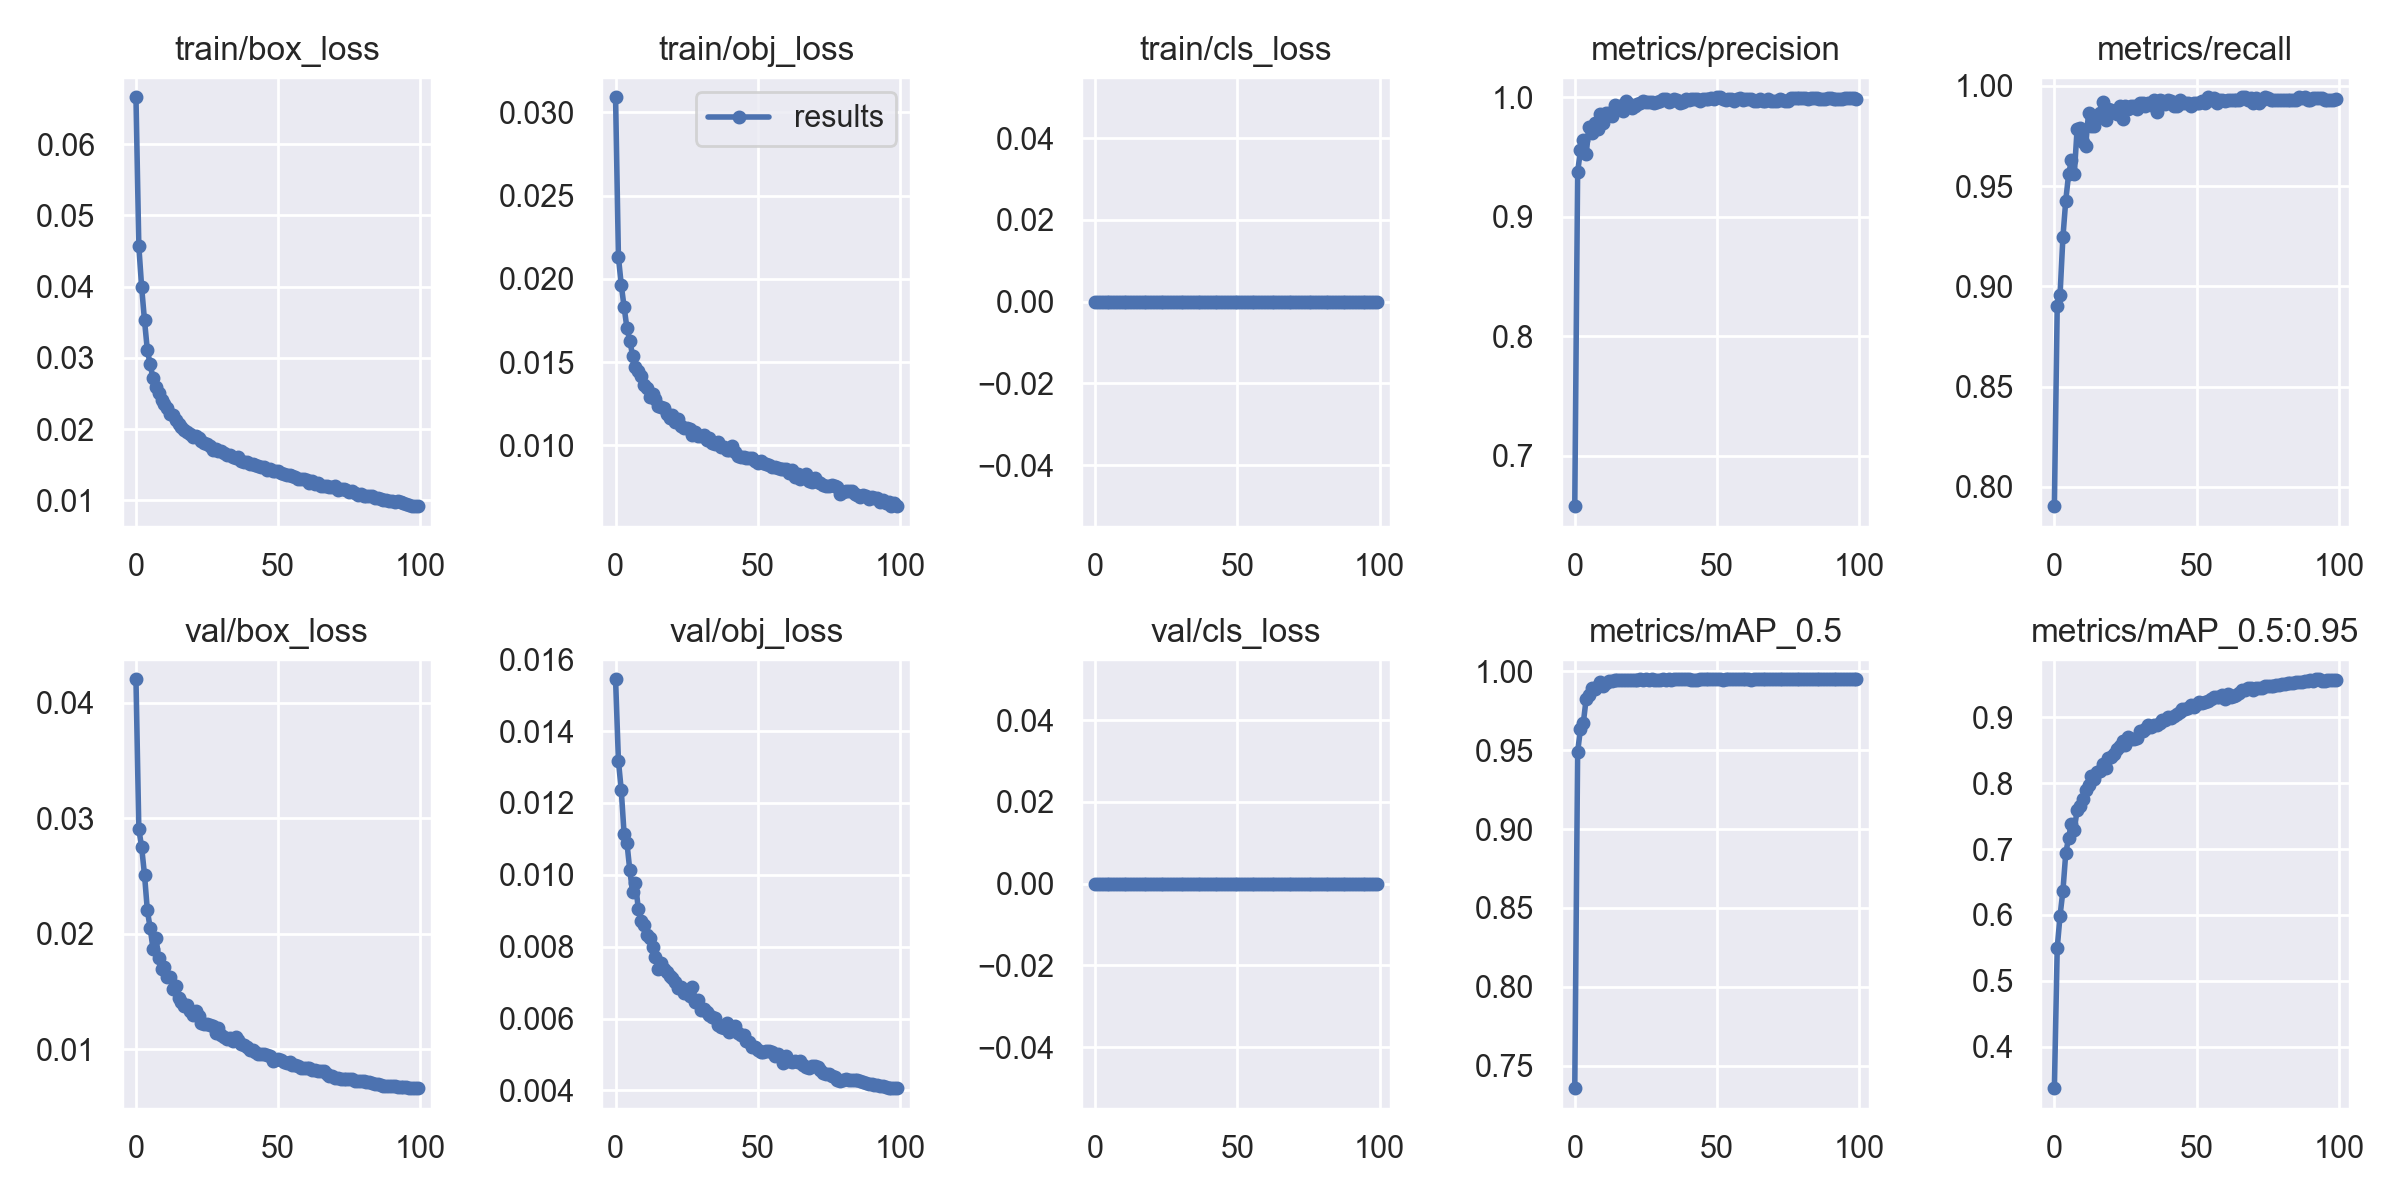
\includegraphics[width=0.94\textwidth]{paper_assets/yolov5_training_results.png}
\caption{Diễn biến loss và các chỉ số đánh giá trong 100 epoch.}
\label{fig:training-curves}
\end{figure}

\subsection{Đánh giá RKNN INT8 trên test set}

Test set gồm 353 ảnh và 353 tệp nhãn YOLO, chứa tổng cộng 872 khuôn mặt. PyTorch, ONNX và RKNN INT8 đều sử dụng cùng ảnh đầu vào 640$\times$640, cùng NMS với ngưỡng IoU 0,60 và cùng cách tính AP tại 10 ngưỡng IoU từ 0,50 đến 0,95. PyTorch được đánh giá bằng \texttt{val.py} của YOLOv5 v7.0 tại commit \texttt{915bbf294bb74c859f0b41f1c23bc395014ea679}. ONNX và RKNN sử dụng cùng phép letterbox với màu đệm 114, chuyển đổi BGR sang RGB và ánh xạ kết quả về ảnh gốc. Các dự đoán có confidence từ 0,001 được dùng để xây dựng đường Precision--Recall; AP được nội suy tại 101 điểm. Precision, Recall và F1 của ONNX cùng RKNN được báo cáo tại confidence 0,50 của ứng dụng, còn Precision và Recall của PyTorch là giá trị tại điểm F1 tối ưu do \texttt{val.py} trả về.

\begin{table}[H]
\centering
\caption{So sánh PyTorch, ONNX và RKNN INT8 trên cùng test set.}
\label{tab:rknn-test}
\small
\begin{tabular}{lrrrrr}
\toprule
Mô hình & Precision & Recall & F1 & mAP@0.5 & mAP@0.5:0.95 \\
\midrule
PyTorch FP32 & 0,99626 & 0,99312 & 0,99469 & 0,99473 & 0,91222 \\
ONNX FP32 & 0,99194 & 0,98853 & 0,99024 & 0,99460 & 0,91322 \\
RKNN INT8 & 0,99194 & 0,98739 & 0,98966 & 0,99454 & 0,89244 \\
\bottomrule
\end{tabular}
\end{table}

PyTorch đạt mAP@0.5 bằng 0,99473 và mAP@0.5:0.95 bằng 0,91222. Sai khác giữa PyTorch và ONNX chỉ là 0,00013 ở mAP@0.5 và 0,00100 ở mAP@0.5:0.95. Tại confidence 0,50 và IoU 0,50, ONNX ghi nhận 862 true positive, 7 false positive và 10 false negative; RKNN INT8 ghi nhận 861 true positive, 7 false positive và 11 false negative. Từ ONNX sang RKNN INT8, mAP@0.5 giảm 0,00006, còn mAP@0.5:0.95 giảm 0,02078. Như vậy, khả năng phát hiện ở IoU 0,50 gần như được bảo toàn, nhưng localization accuracy giảm rõ hơn tại các ngưỡng IoU cao.

\begin{figure}[H]
\centering
\begin{tikzpicture}[x=6.2cm,y=4.2cm,font=\small]
\draw[->] (0,0)--(1.08,0) node[right]{mAP};
\foreach \x in {0,0.2,0.4,0.6,0.8,1.0}{\draw (\x,0.04)--(\x,-0.04) node[below]{\x};}
\fill[blue!65] (0,1.55) rectangle (0.99460,1.82);
\fill[teal!70] (0,1.18) rectangle (0.99454,1.45);
\fill[blue!65] (0,0.63) rectangle (0.91322,0.90);
\fill[teal!70] (0,0.26) rectangle (0.89244,0.53);
\node[anchor=east] at (-0.02,1.685){ONNX, IoU 0,50};
\node[anchor=east] at (-0.02,1.315){RKNN, IoU 0,50};
\node[anchor=east] at (-0.02,0.765){ONNX, IoU 0,50:0,95};
\node[anchor=east] at (-0.02,0.395){RKNN, IoU 0,50:0,95};
\end{tikzpicture}
\caption{So sánh mAP của ONNX FP32 và RKNN INT8 trên cùng 353 ảnh thuộc test set; PyTorch FP32 đạt mAP@0.5:0.95 bằng 0,91222.}
\label{fig:accuracy-comparison}
\end{figure}

\subsection{Benchmark detector}

Hai nền tảng được benchmark với từng ảnh riêng lẻ ở kích thước 640$\times$640. Trên mỗi nền tảng, 20 warm-up runs được thực hiện trước 100 benchmark runs. Latency của từng run được đo bằng \texttt{CLOCK\_MONOTONIC}. Phía PC sử dụng ONNX Runtime 1.23.2 trên CPU Intel Core i5-1135G7 (4 nhân, 8 luồng). Phía Luckfox đo riêng NPU inference bằng \texttt{rknn\_run} và bước post-processing trên RV1106, Linux 5.10.160, ARM 32 bit.

Thời gian trong Bảng~\ref{tab:bench} không bao gồm thu ảnh camera, chuẩn bị ảnh đầu vào, nhận diện danh tính, phân biệt khuôn mặt thật với ảnh giả, vẽ thông tin, mã hóa H.264 hoặc truyền mạng. Vì vậy, cột FPS suy ra chỉ biểu diễn tốc độ của detector. Để phản ánh tốc độ thực tế, luồng RTSP được đọc liên tục trong 10 giây bằng FFprobe; kết quả ghi nhận 58 frame, tương ứng 5,8 FPS cho toàn bộ ứng dụng.

\begin{table}[H]
\centering
\caption{Benchmark detector với 20 warm-up runs và 100 benchmark runs.}
\label{tab:bench}
\small
\begin{tabular}{>{\raggedright\arraybackslash}p{42mm}rrrrr}
\toprule
Platform / stage & Mean (ms) & Std (ms) & p50 (ms) & p95 (ms) & FPS suy ra \\
\midrule
PC --- ONNX Runtime CPU & 136,46 & 102,58 & 125,37 & 188,56 & 7,33 \\
RV1106 --- NPU inference & 104,10 & 0,97 & 103,98 & 105,41 & 9,61 \\
RV1106 --- post-processing & 3,85 & 0,43 & 3,61 & 4,64 & --- \\
RV1106 --- detector pipeline & 107,95 & 0,97 & 107,71 & 109,22 & 9,26 \\
RTSP --- end-to-end (10 s) & --- & --- & --- & --- & 5,80 \\
\bottomrule
\end{tabular}
\end{table}

\begin{figure}[H]
\centering
\begin{tikzpicture}[x=0.055cm,y=0.8cm,font=\small]
\draw[->] (0,0)--(205,0) node[right]{ms};
\foreach \x in {0,50,100,150,200}{\draw (\x,0.08)--(\x,-0.08) node[below]{\x};}
\fill[blue!65] (0,1.8) rectangle (136.46,2.35); \node[anchor=east] at (-3,2.08){PC Mean}; \node[anchor=west] at (138,2.08){136,46};
\fill[teal!70] (0,1.0) rectangle (107.95,1.55); \node[anchor=east] at (-3,1.28){RV1106 Mean}; \node[anchor=west] at (109.5,1.28){107,95};
\fill[orange!80] (0,0.2) rectangle (188.56,0.75); \node[anchor=east] at (-3,0.48){PC p95}; \node[anchor=west] at (190,0.48){188,56};
\end{tikzpicture}
\caption{So sánh độ trễ ONNX/CPU và RKNN/NPU.}
\label{fig:latency-comparison}
\end{figure}

RKNN trên NPU của Luckfox giảm 20,89\% Mean latency so với ONNX trên CPU của PC và cho tốc độ lý thuyết cao hơn khoảng 1,26 lần. Std của toàn bộ detector trên RV1106 là 0,97 ms, trong khi trên PC là 102,58 ms và có một lượt kéo dài tới 886,78 ms. Các giá trị p50 và p95 được báo cáo cùng Mean để mô tả phân bố latency. Trong điều kiện đo đã thiết lập, RV1106 có latency thấp hơn và ổn định hơn.

\subsection{Đánh giá chức năng}

Mô hình RKNN INT8 đã được nạp và chạy trực tiếp trong chương trình C++ biên dịch cho kiến trúc ARM 32 bit của Luckfox. Kiểm thử tích hợp xác nhận các chức năng gồm phát video H.264 720$\times$480 qua RTSP, xem hình qua HTTP/MJPEG, đăng ký và xóa nhân viên, lưu cơ sở dữ liệu, hiển thị tên trên bounding box và ghi sự kiện sau khi phân biệt khuôn mặt thật với ảnh giả trong ba khung hình liên tiếp.

Kết quả trên thiết bị cho thấy mô hình RKNN có thể phát hiện khuôn mặt liên tục, cung cấp bounding box cho bước nhận diện và duy trì đồng thời RTSP cùng giao diện web. Việc đánh giá trên test set được thực hiện ở chế độ mô hình phát hiện độc lập để loại ảnh hưởng của FaceNet, phân biệt khuôn mặt thật với ảnh giả, mã hóa video và truyền mạng khỏi metric phát hiện.

\section{Conclusion and future works}

Nghiên cứu đã hoàn thiện quy trình từ 3.536 ảnh gốc, bộ dữ liệu 9.194 ảnh sau data augmentation, đến YOLOv5s và ứng dụng điểm danh xFace trên RV1106. Trên cùng test set gồm 353 ảnh, PyTorch FP32, ONNX FP32 và RKNN INT8 lần lượt đạt mAP@0.5:0.95 là 0,91222, 0,91322 và 0,89244. RKNN INT8 đạt Precision 0,99194, Recall 0,98739 và mAP@0.5 bằng 0,99454. Tổng latency của detector trên NPU là 107,95 ms, với p95 là 109,22 ms. So với ONNX trên CPU của PC, Mean latency giảm 20,89\% và Std cũng thấp hơn. Luồng RTSP thực tế đạt 5,8 FPS khi tính cả phát hiện, nhận diện, phân biệt khuôn mặt thật--giả, vẽ kết quả và mã hóa video. Các kết quả này xác nhận mô hình YOLOv5s do nhóm train đã được chuyển đổi và tích hợp thành công vào ứng dụng Edge AI hoạt động trực tiếp trên thiết bị nhúng.

Mô hình phát hiện chỉ trả về bounding box, không dự đoán các landmark như mắt, mũi và khóe miệng; vì vậy chất lượng căn chỉnh có thể giảm khi khuôn mặt nghiêng nhiều.

Các hướng tiếp theo gồm mở rộng dữ liệu theo góc nhìn và điều kiện chiếu sáng; dự đoán trực tiếp landmark khuôn mặt; lưu lịch sử điểm danh lâu dài; và kiểm thử hệ thống trong thời gian dài ở môi trường sử dụng thực tế.

\begin{thebibliography}{9}
\bibitem{yolov5} Ultralytics, \emph{YOLOv5}, phiên bản v7.0, 2022. \url{https://github.com/ultralytics/yolov5}
\bibitem{facenet} F. Schroff, D. Kalenichenko và J. Philbin, ``FaceNet: A Unified Embedding for Face Recognition and Clustering,'' \emph{CVPR}, 2015.
\bibitem{rknn} Rockchip, \emph{RKNN-Toolkit2 and RKNPU Model Zoo}, tài liệu và mã nguồn công cụ triển khai mạng nơ-ron trên RKNPU.
\bibitem{roboflow} Roboflow, \emph{Face Detection Dataset, version 2}, giấy phép CC BY 4.0, truy cập trong quá trình thực nghiệm năm 2026.
\end{thebibliography}

\end{document}
